\documentclass{article}
\usepackage[utf8]{inputenc}
\usepackage[english]{babel}
\usepackage[font=small,labelfont=bf]{caption}
\usepackage{geometry}
\usepackage{natbib}
\usepackage{pxfonts}
\usepackage{graphicx}
\usepackage{newfloat}
\usepackage{setspace}
\usepackage{hyperref}
\usepackage{placeins}
\usepackage{rotating}

\doublespacing

\newcommand{\argmax}{\mathop{\mathrm{argmax}}\limits}
\newcommand{\argmin}{\mathop{\mathrm{argmin}}\limits}

\newcommand{\demo}{1}

\title{\textit{Supplementary materials for}: Feature and order manipulations in
a free recall task affect memory for current and future lists}

\author{Jeremy R. Manning\textsuperscript{1, *}, Emily C.
Whitaker\textsuperscript{1}, Paxton C. Fitzpatrick\textsuperscript{1},
\\Madeline R. Lee\textsuperscript{1}, Allison M. Frantz\textsuperscript{1},
Bryan J. Bollinger\textsuperscript{1},\\Darya Romanova\textsuperscript{1},
Campbell E. Field\textsuperscript{1}, and Andrew C. Heusser\textsuperscript{1,
2}\\\textsuperscript{1}Dartmouth College\\\textsuperscript{2}Akili
Interactive\\\textsuperscript{*}Corresponding author:
jeremy.r.manning@dartmouth.edu}

\date{}

\begin{document}

\renewcommand{\figurename}{Supplementary Figure}

%\begin{titlepage}
%  \maketitle
%  \thispagestyle{empty}
%\end{titlepage}

\setcounter{equation}{0}
\setcounter{figure}{0}
\setcounter{table}{0}
\setcounter{page}{1}
\setcounter{section}{0}
\makeatletter
\renewcommand{\theequation}{S\arabic{equation}}
\renewcommand{\thefigure}{S\arabic{figure}}
\renewcommand{\bibnumfmt}[1]{[S#1]}
\renewcommand{\citenumfont}[1]{S#1}

\maketitle

\begin{figure}[p] \centering
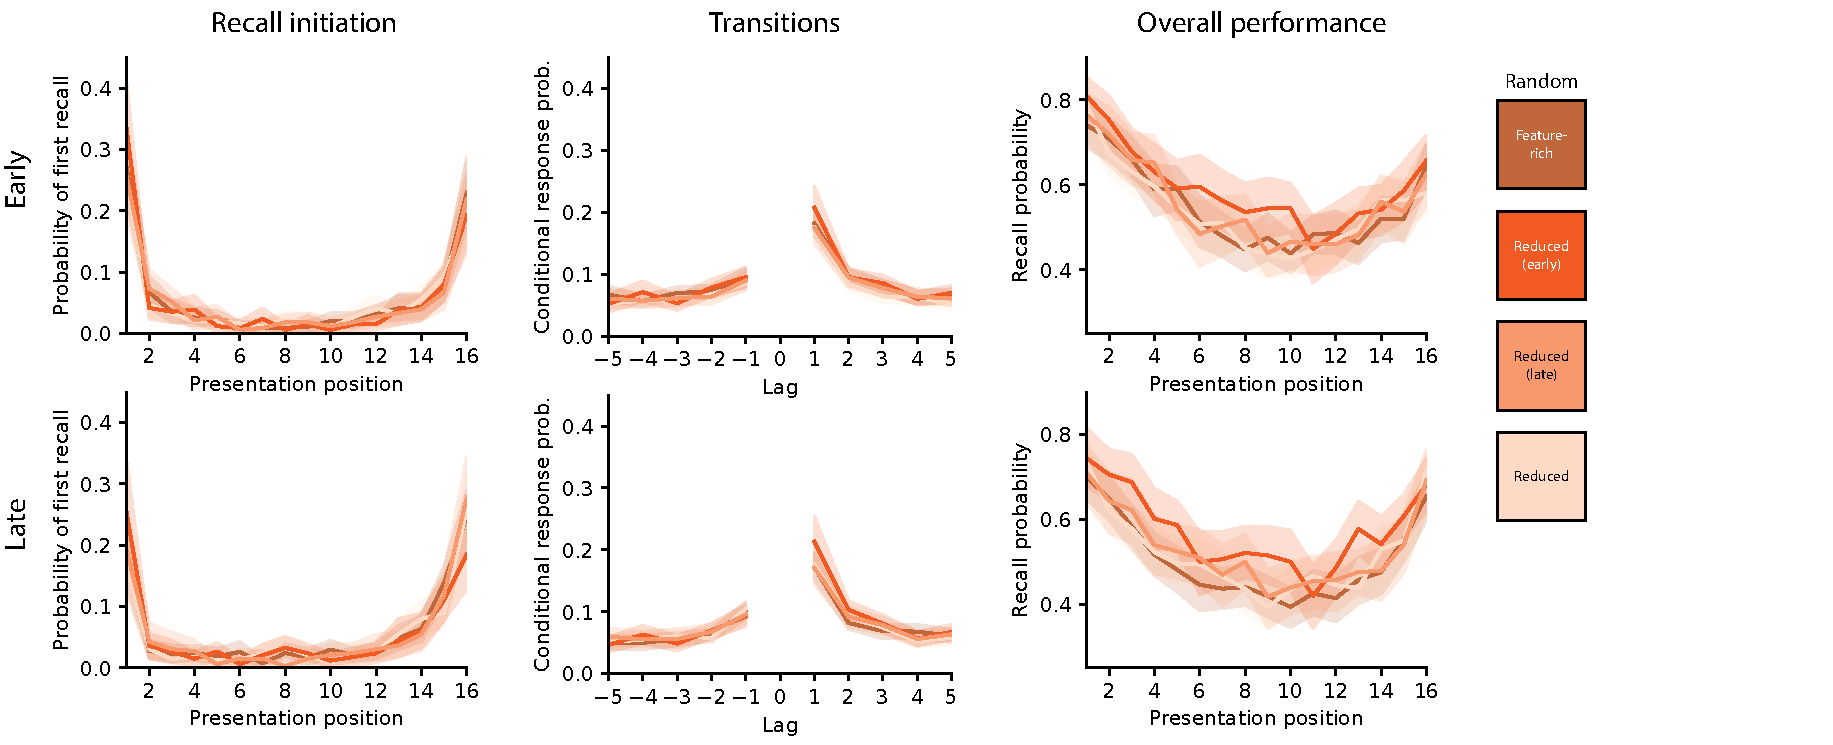
\includegraphics[width=\textwidth]{figures/recall_dynamics_random}

\caption{\textbf{Recall dynamics in feature rich free recall (random conditions).} \textbf{Left panels.} The probabilities of
initiating recall with each word are plotted as a function of presentation
position. \textbf{Middle panels.} The conditional probabilities of recalling
each word are plotted as a function of the relative position (Lag) to the words
recalled just-prior. \textbf{Right panels.} The overall probabilities of
recalling each word are plotted as a function of presentation position.
\textbf{All panels.} Error ribbons denote bootstrap-estimated 95\% confidence
intervals (calculated across participants). Top panels display the recall
dynamics for early (order manipulation) lists in each condition (color). Bottom
panels display the recall dynamics for late (randomly ordered) lists.}

    \label{fig:recall-dynamics-random}
\end{figure}

\begin{figure}[p] \centering
    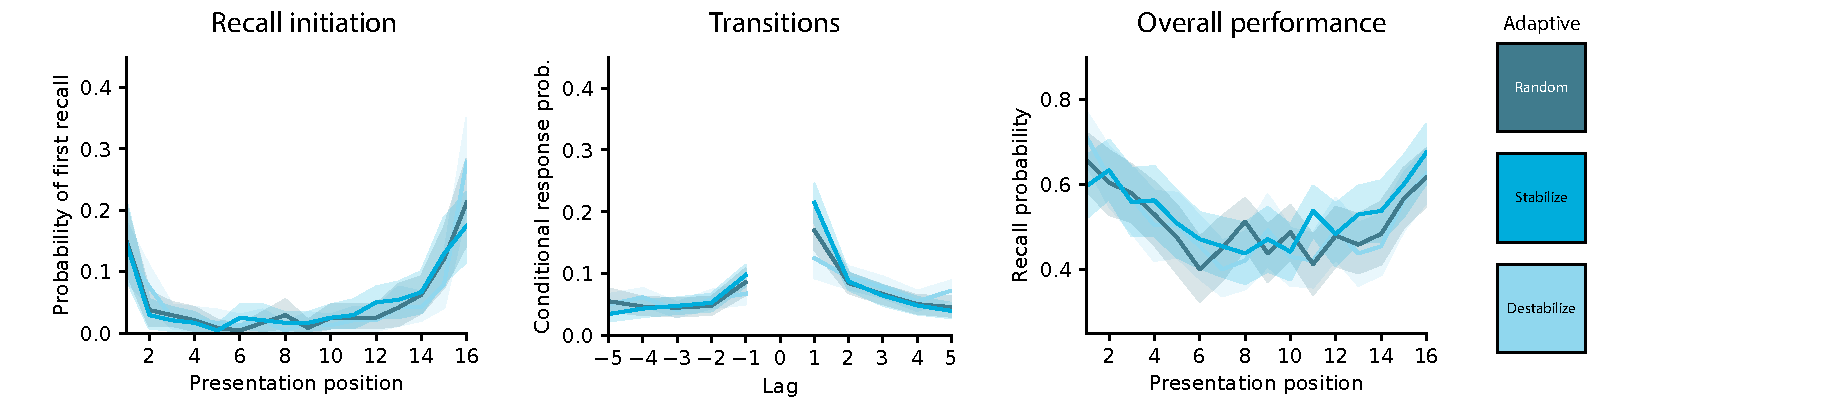
\includegraphics[width=\textwidth]{figures/recall_dynamics_adaptive}
    
    \caption{\textbf{Recall dynamics in feature rich free recall (adaptive conditions).} \textbf{Left panel.} The probabilities of
    initiating recall with each word are plotted as a function of presentation
    position. \textbf{Middle panel.} The conditional probabilities of recalling
    each word are plotted as a function of the relative position (Lag) to the words
    recalled just-prior. \textbf{Right panel.} The overall probabilities of
    recalling each word are plotted as a function of presentation position.
    \textbf{All panels.} Error ribbons denote bootstrap-estimated 95\% confidence
    intervals (calculated across participants). Condition is denoted by color.}
    
        \label{fig:recall-dynamics-adaptive}
    \end{figure}


\begin{figure}[tp] \centering
    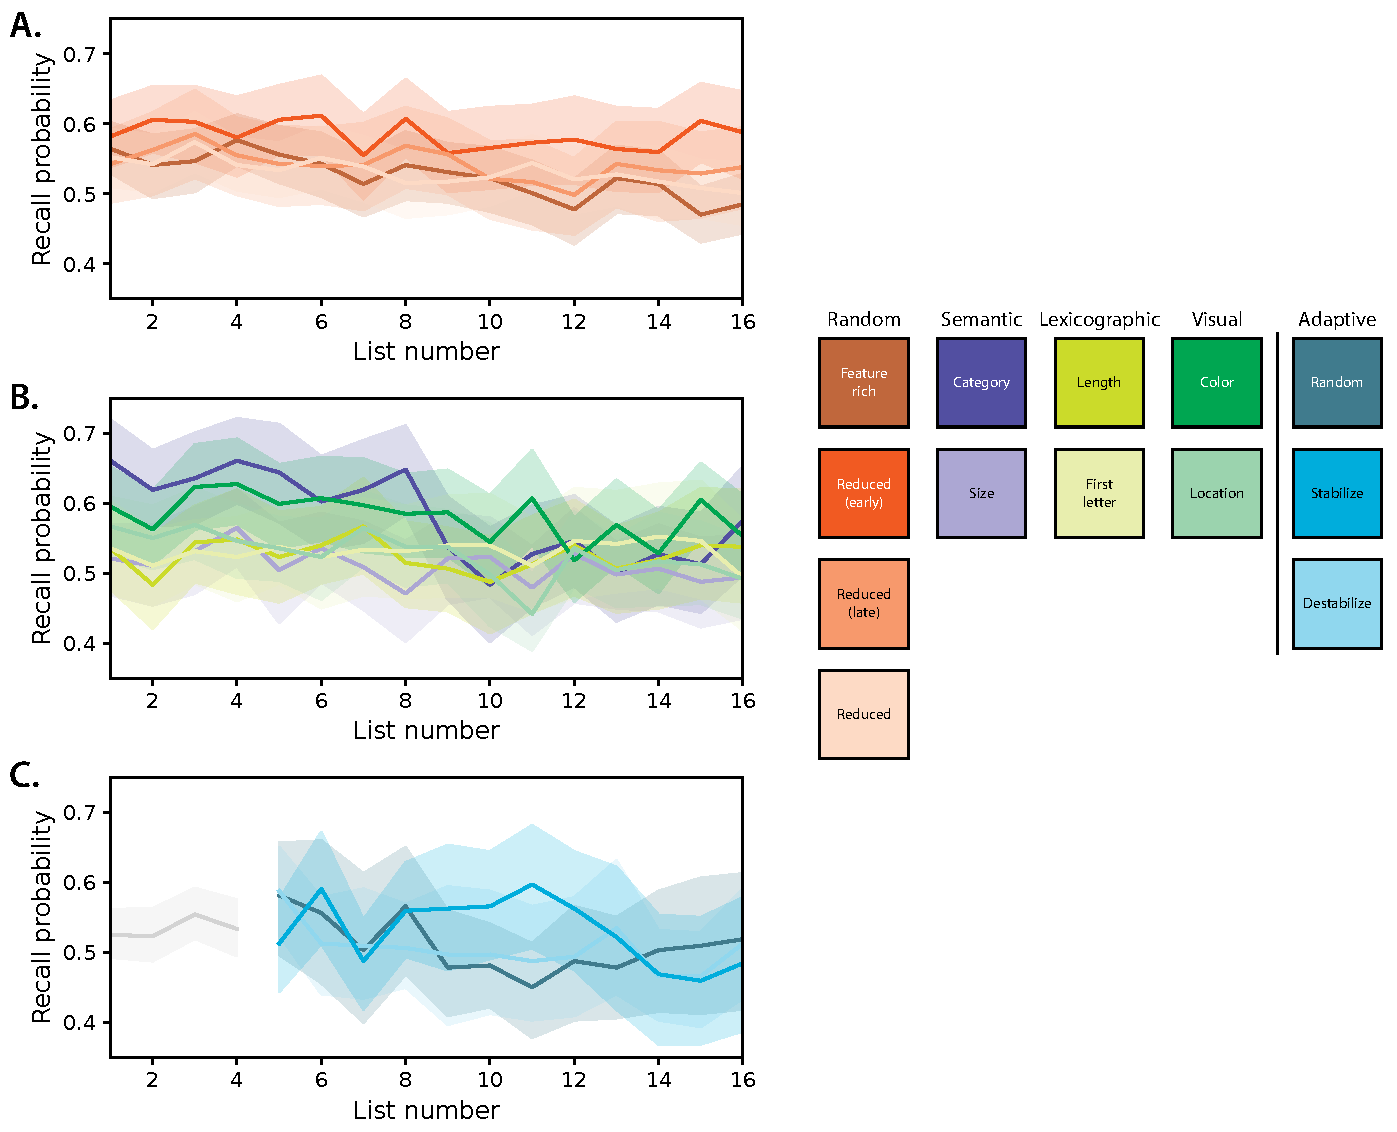
\includegraphics[width=0.75\textwidth]{figures/accuracy_by_list}
    
\caption{\textbf{Recall accuracy by study list number.} Each panel displays the
average recall accuracy (across participants) as a function of the number of
studied lists for the random conditions (\textbf{A.}), order manipulation
conditions (\textbf{B.}), and adaptive conditions (\textbf{C.}). The conditions
are denoted by color. Note that the first four lists in all of the ``adaptive''
conditions were ordered randomly to compute a baseline fingerprint for each
participant prior to initiating the adaptive ordering procedure. \textbf{All
panels.} All error ribbons denote bootstrap-estimated 95\% confidence
intervals, calculated across participants.} 
\label{fig:accuracy-by-list}

\end{figure}


\begin{figure}[tp] \centering
    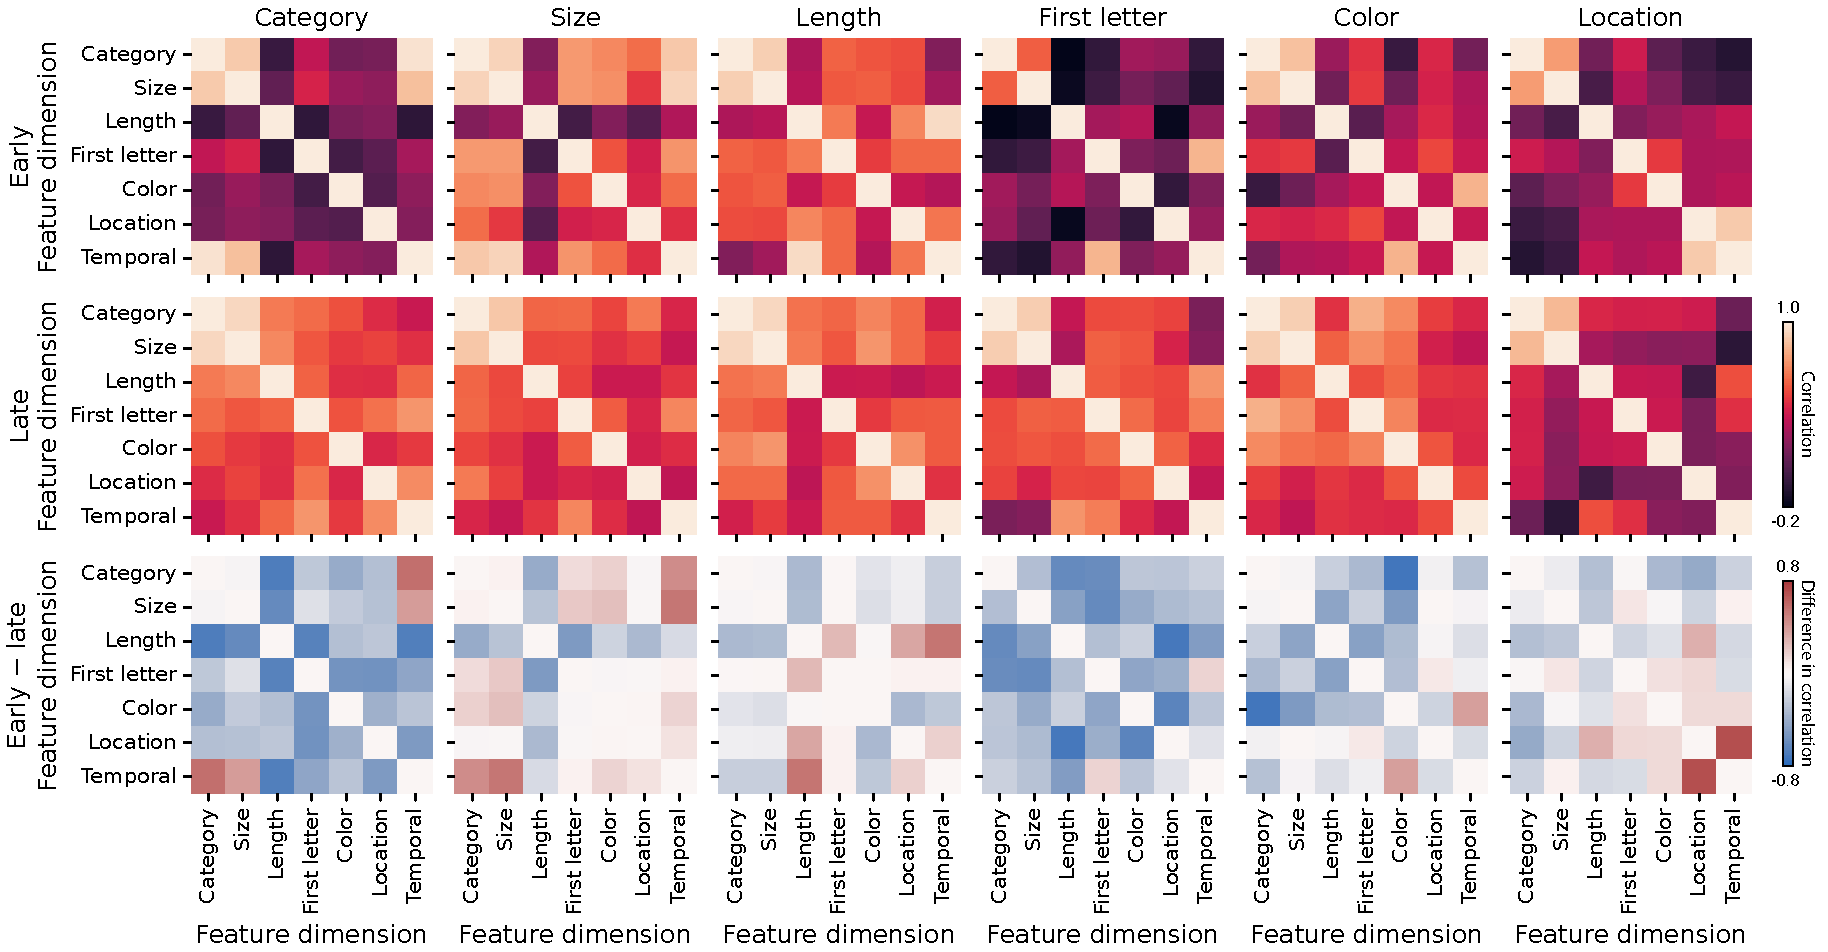
\includegraphics[width=\textwidth]{figures/clustering_correlations}
    
    \caption{\textbf{Correlations between feature clustering scores (order manipulation conditions).}  Each column reflects one experimental condition.  The matrices in the top and middle
    rows display across-participant correlations between clustering scores for each feature dimension (top: order manipulation lists; middle: randomly ordered lists).  The matrices
    in the bottom rows display the differences between the top and middle rows.}
        \label{fig:clustering-correlations}
\end{figure}


\begin{figure}[tp] \centering
    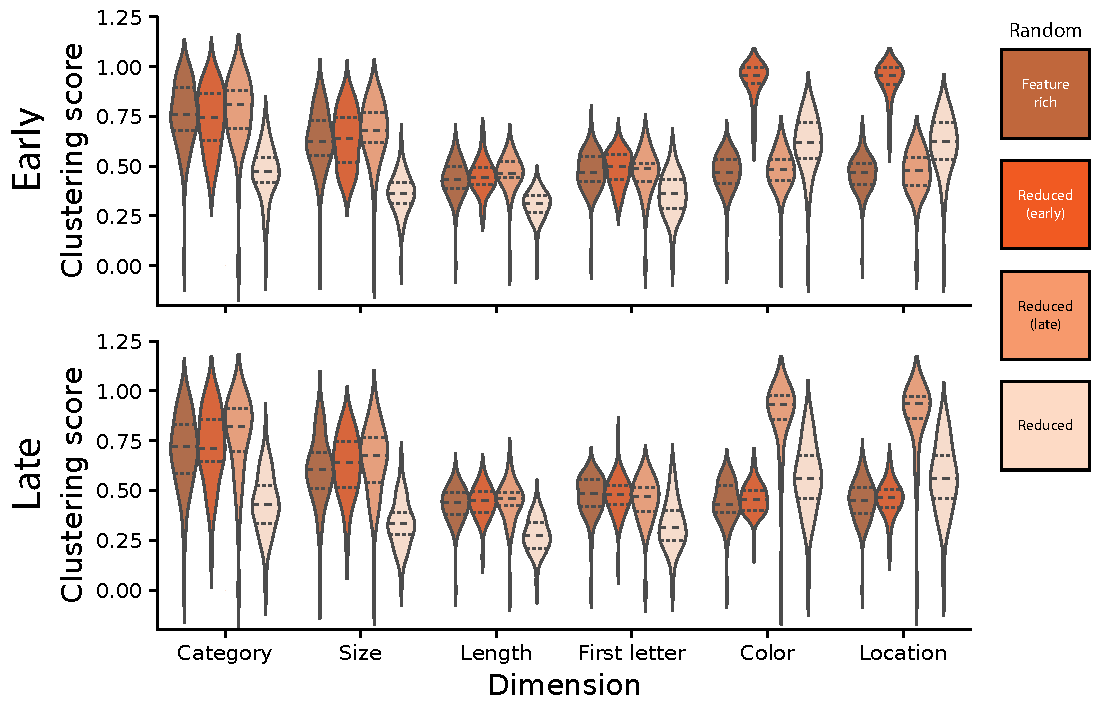
\includegraphics[width=\textwidth]{figures/fingerprints_random}
    
\caption{\textbf{Memory ``fingerprints'' (random conditions).} The
across-participant clustering scores for each feature type ($x$-axis) are
displayed for each experimental condition (color), separately for early (top)
and late (bottom) lists. Error bars denote bootstrap-estimated 95\% confidence
intervals.}

\label{fig:fingerprints-random} \end{figure}
    
\begin{figure}[tp] \centering
    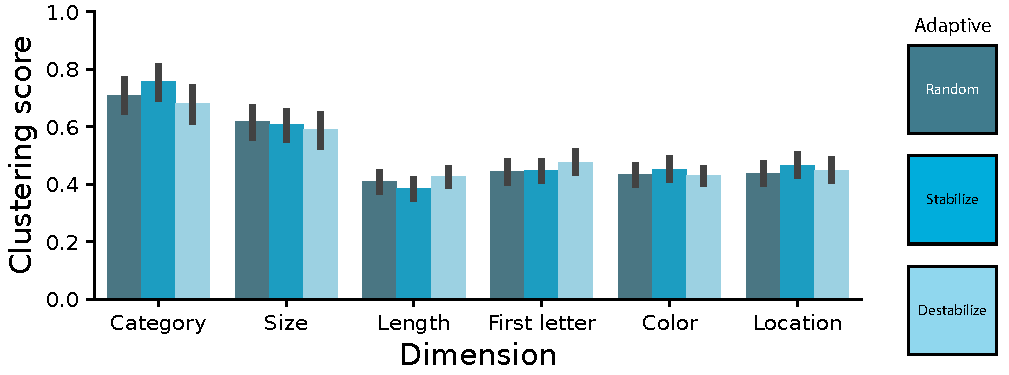
\includegraphics[width=\textwidth]{figures/fingerprints_adaptive}
    
\caption{\textbf{Memory ``fingerprints'' (adaptive conditions).} The
across-participant clustering scores for each feature type ($x$-axis) are
displayed for each experimental condition (color). Error bars denote
bootstrap-estimated 95\% confidence intervals.}

\label{fig:fingerprints-adaptive} \end{figure}


\begin{sidewaysfigure}
    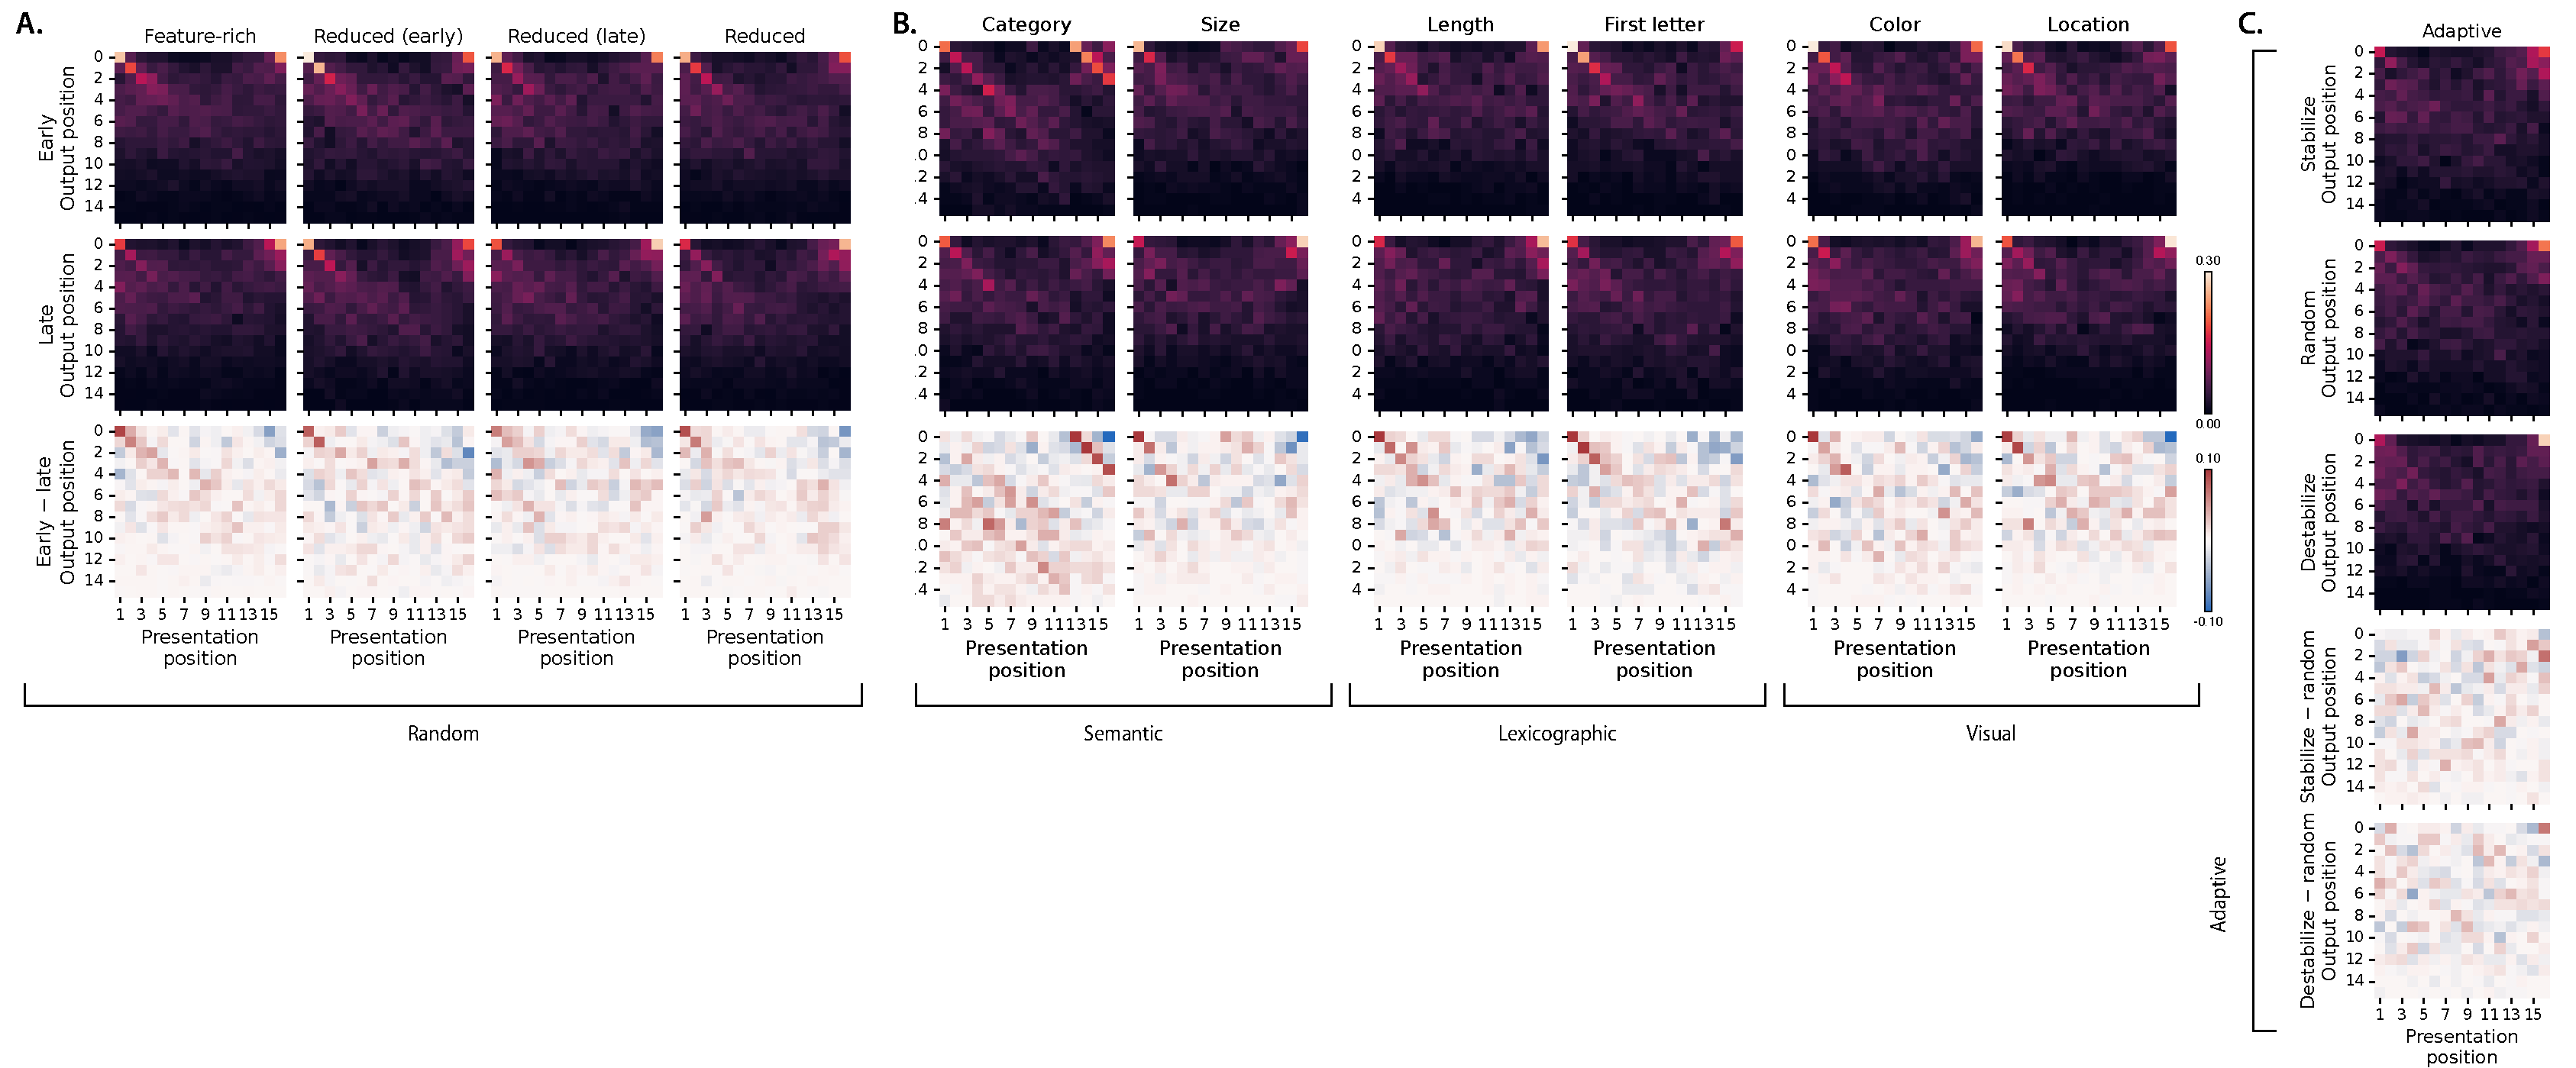
\includegraphics[width=\textwidth]{figures/pnr_matrices}

    \caption{\textbf{Probability of $n$\textsuperscript{th} recall matrices.}
    Each sub-panel displays the average probability of recalling the given word
    (Presentation position, matrix column) at the given output position (matrix
    row); color denotes the probability. \textbf{A. Random conditions.} The top
    rows of matrices display data from early (order manipulation) lists, the
    middle rows of matrices display data from late (randomly ordered) lists,
    and the bottom rows of matrices display the differences between the
    matrices in the top and middle rows. Panel columns denote experimental
    conditions. \textbf{B. Order manipulation conditions.} The matrices are
    displayed in the same format as those in Panel A. Panel columns are
    organized by feature type (semantic, lexicographic, or visual). \textbf{C.
    Adaptive conditions.} The sub-panels are displayed in the same formats as
    Panels A and B, but here the matrices and contrasts (indicated in $y$-axis
    labels) reflect different list manipulation conditions.}

    \label{fig:pnr}
\end{sidewaysfigure}

\begin{figure}[tp] \centering
    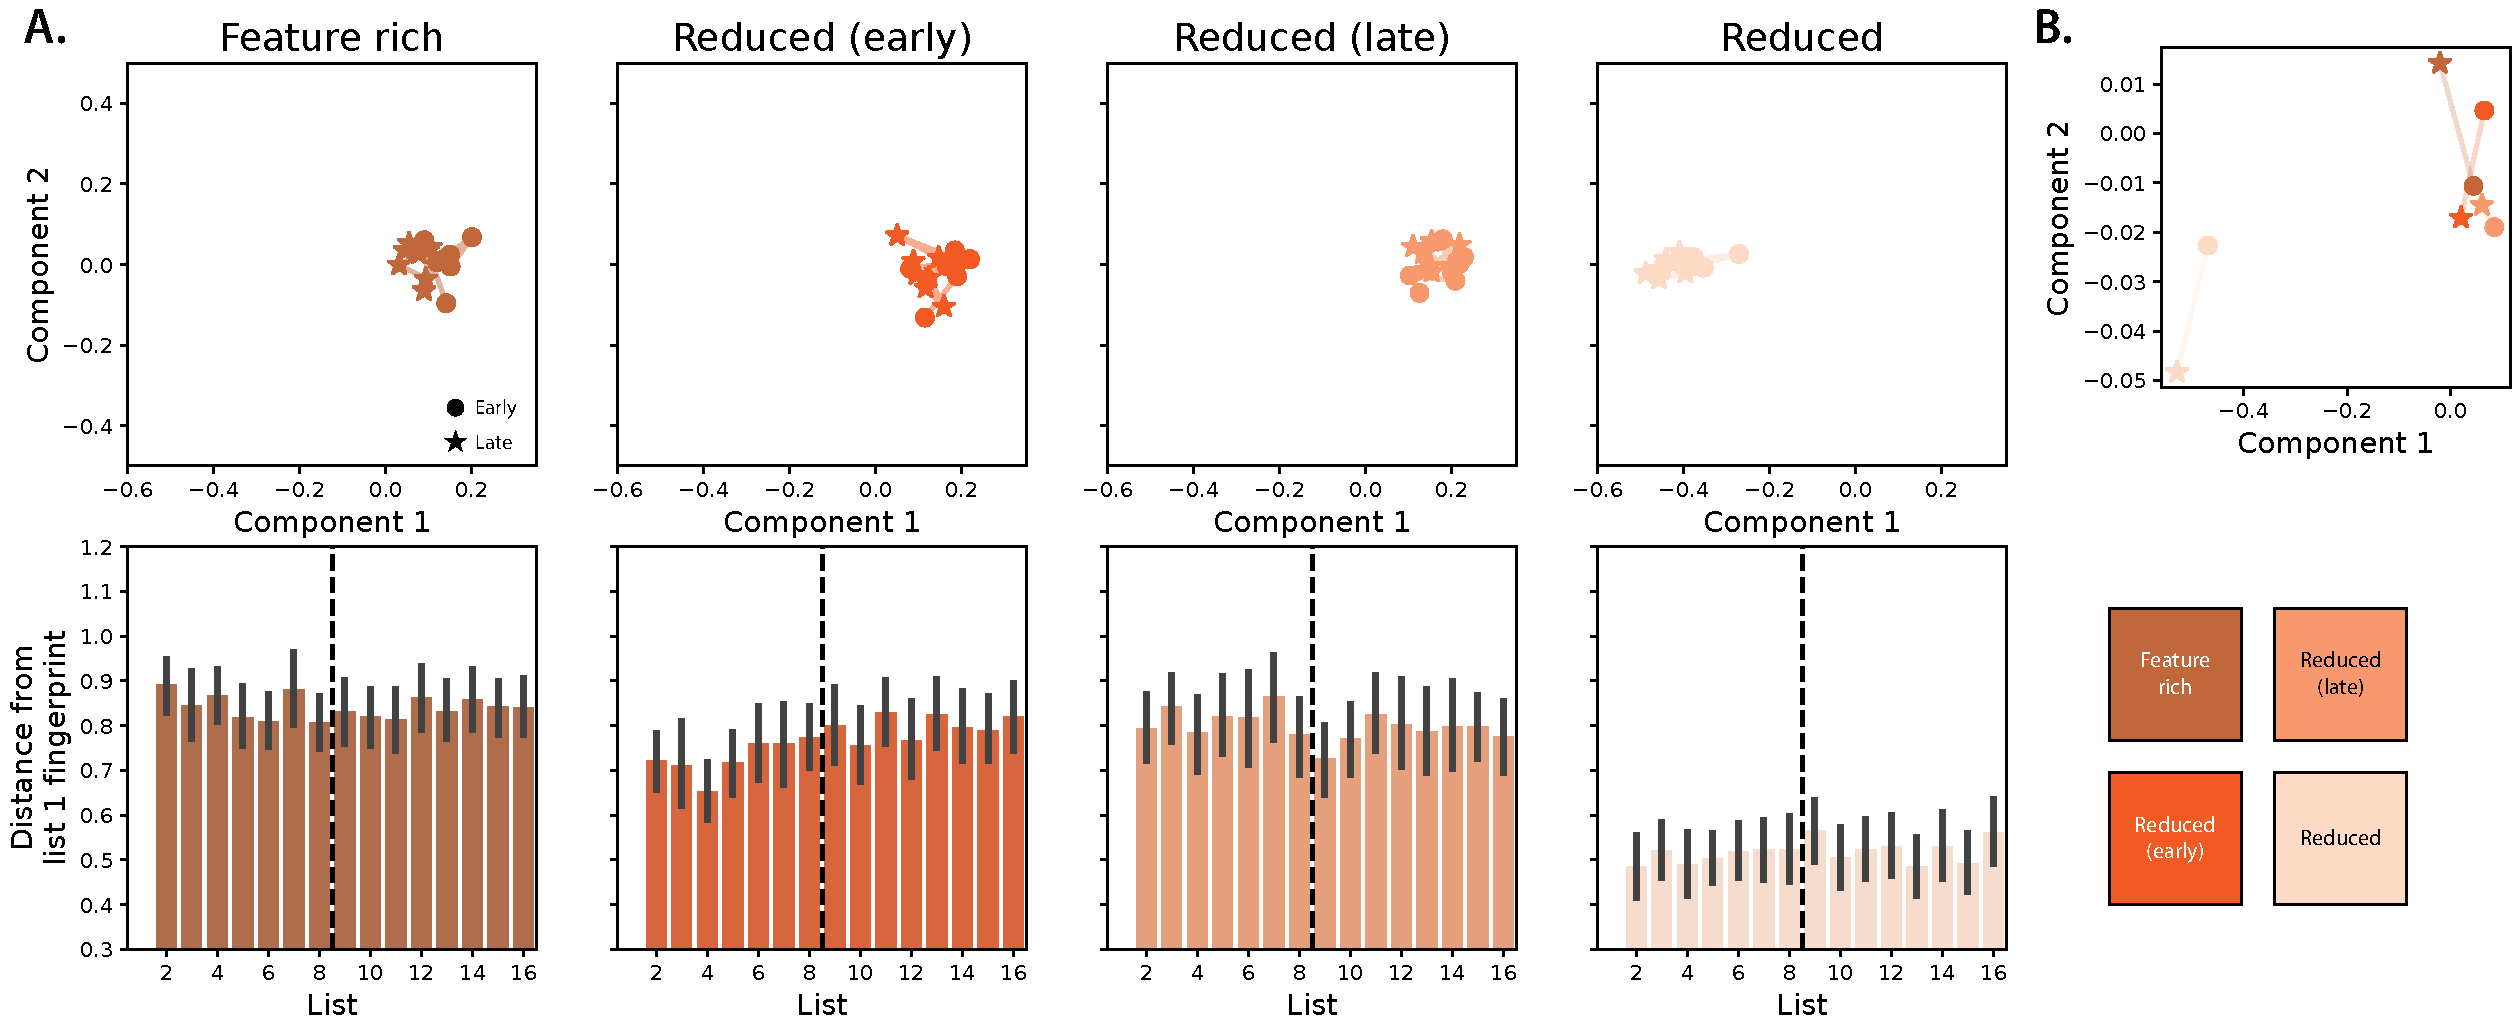
\includegraphics[width=\textwidth]{figures/fingerprint_trajectories_random}
    
    \caption{\textbf{Memory fingerprint dynamics (random conditions).}
    \textbf{A.} Each column (and color) reflects an experimental condition. In
    the top panels, each marker displays a 2D projection of the
    (across-participant) average memory fingerprint for one list. Early lists
    are denoted by circles and late lists are denoted by stars. All of the
    fingerprints (across all conditions and lists) are projected into a common
    space. The bar plots in the bottom panels display the Euclidean distances
    of the per-list memory fingerprints to the list 0 fingerprint, for each
    condition. Error bars denote bootstrap-estimated 95\% confidence intervals.
    The dotted vertical lines denote the boundaries between early and late
    lists. \textbf{B.} In this panel, the fingerprints for early (circle) and
    late (star) lists are averaged across lists and participants before
    projecting the fingerprints into a (new) 2D space.} \label{fig:fingerprint-trajectories-random}
    
    \end{figure}

    \begin{figure}[tp] \centering
        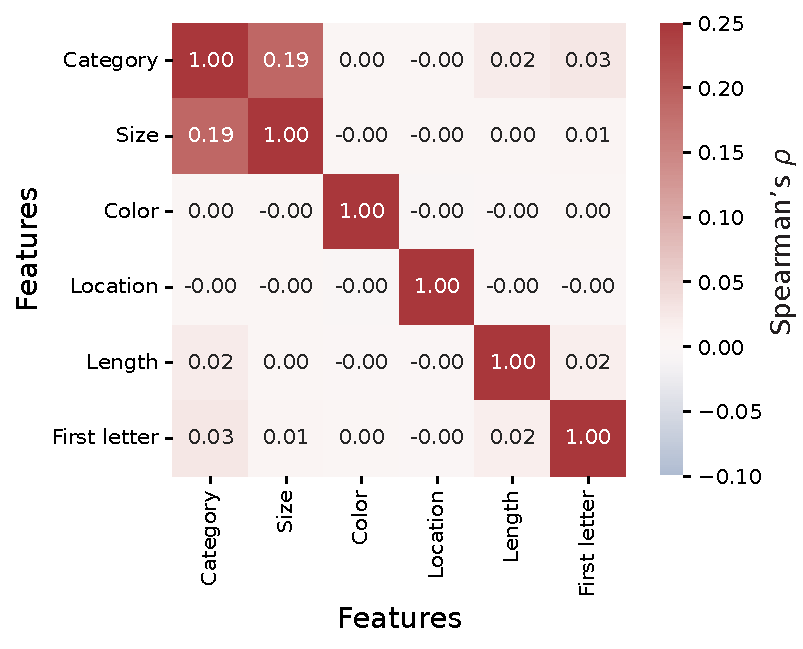
\includegraphics[width=0.6\textwidth]{figures/feature_correlations}
        
        \caption{\textbf{Correlations between features.} Within each list, for each participant, we
        computed the set of distances between each pair of words, along each feature dimension.  We
        then combined these pairwise distances across all lists and participants, and computed the
        Spearman correlation between the distances for each pair of feature dimensions.  The correlation
        coefficients are displayed in the heatmap, annotated with each cell's value.} \label{fig:feature-correlations}
        
        \end{figure}

% accuracy by list (list order effects)


% correlations between different types of clustering

%\newpage
%\renewcommand{\refname}{Supplementary references}
%\bibliographystyle{apa}
%\bibliography{CDL-bibliography/cdl}



\end{document}
